\chapter{RESULTADOS}
\label{cap:resultados}

Este capítulo presenta los resultados experimentales de GBMARL siguiendo el orden de construcción del marco: la calibración del simulador (Sección~\ref{sec:res-calibracion}), la validación del entorno y la convergencia del aprendizaje (Sección~\ref{sec:res-aprendizaje}), la comparación frente a las líneas base con la métrica auditada (Sección~\ref{sec:res-comparacion}), el mecanismo de la política aprendida (Sección~\ref{sec:res-mecanismo}), la ablación del crítico centralizado (Sección~\ref{sec:res-ablacion}) y el análisis de sensibilidad (Sección~\ref{sec:res-sensibilidad}). La interpretación de estos hallazgos y sus implicaciones se desarrollan en el capítulo siguiente.

\section{Calibración del simulador}
\label{sec:res-calibracion}

La corrección del cruce entre GDSC2 y DepMap (normalización de claves en ambos lados) recuperó \textbf{34 líneas celulares de glioblastoma} con ensayos de sensibilidad a temozolomida, de las cuales \textbf{24} cuentan con anotación genómica completa. Esto contrasta con las 6 líneas que recuperaba la versión defectuosa del cruce por nombre, lo que confirma que aquel valor era un artefacto de mapeo y no una limitación real de los datos.

De estos ensayos se derivó una concentración inhibitoria media de la población sensible $\mathrm{IC50}_S \approx 0{,}36$ y de la población resistente $\mathrm{IC50}_R \approx 3{,}27$, es decir, una brecha de sensibilidad de aproximadamente $9\times$. El techo de muerte celular, anclado a literatura mediante la razón muerte-crecimiento, resultó en $\delta_S^{\max} = 0{,}30$ y $\delta_R^{\max} = 0{,}15$. Un hallazgo relevante de la calibración es que estos valores caracterizan a la temozolomida como un fármaco débil \emph{in vitro}, coherente con el carácter clínicamente refractario del glioblastoma. La Figura~\ref{fig:dynamics} muestra la dinámica de referencia del simulador calibrado bajo distintos regímenes de dosis.

\begin{figure}[H]
\centering
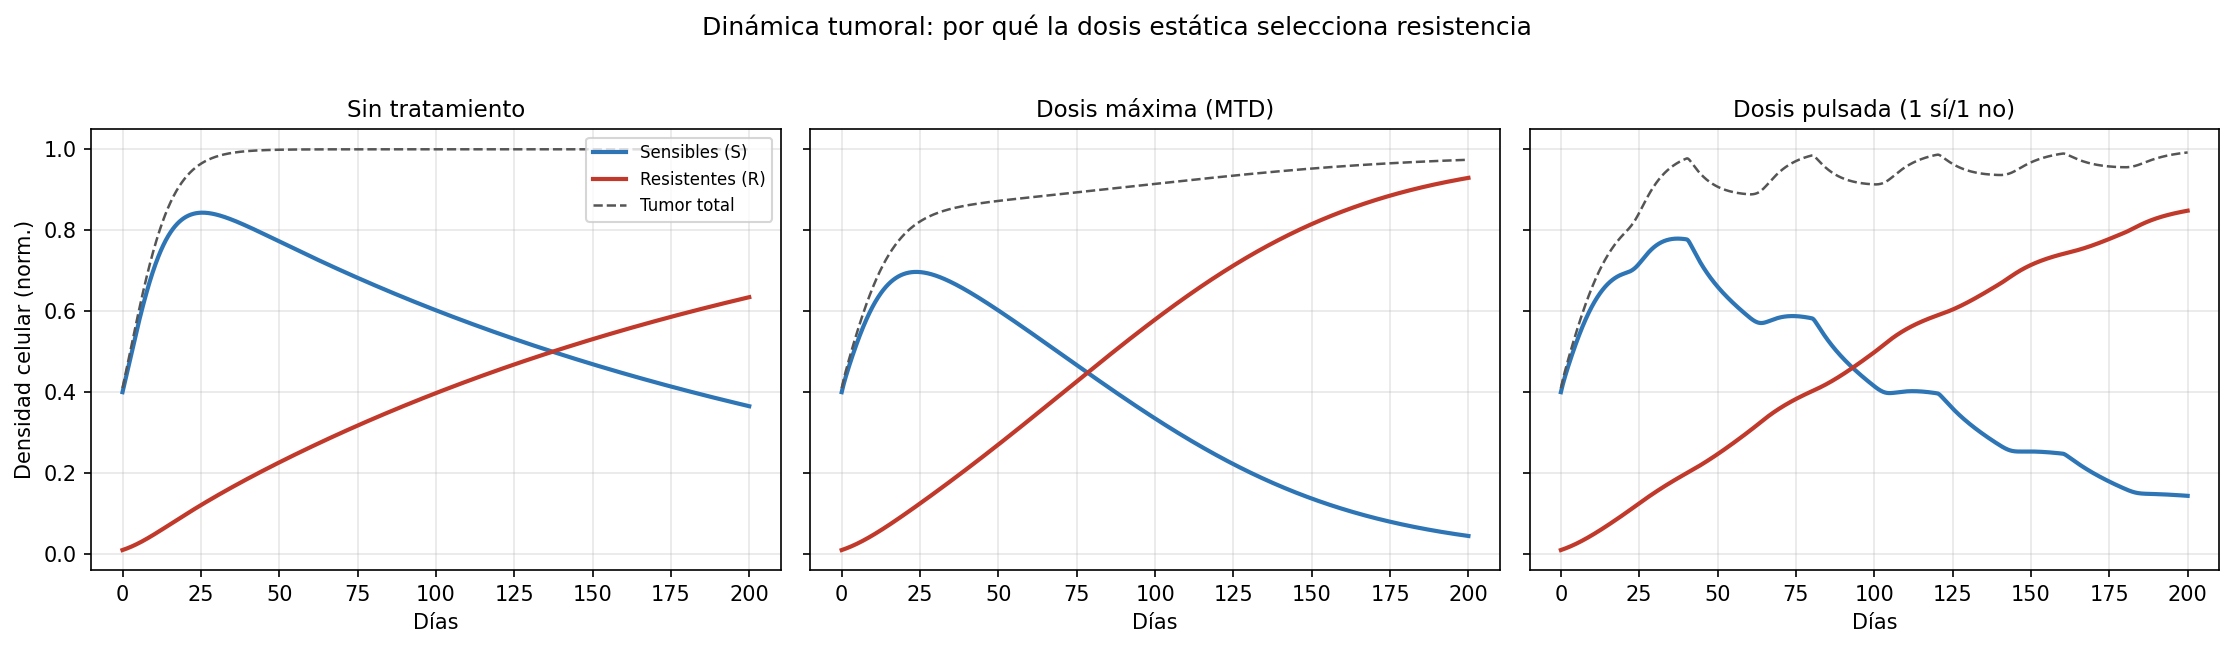
\includegraphics[width=0.85\textwidth]{images/dynamics_baseline.png}
\caption{Dinámica de referencia del simulador calibrado: evolución de las poblaciones sensible y resistente bajo distintos regímenes de dosificación.}
\label{fig:dynamics}
\end{figure}

\section{Validación del entorno y convergencia del aprendizaje}
\label{sec:res-aprendizaje}

Siguiendo la estrategia de validación incremental, se entrenó primero un agente único con PPO contra un tumor de comportamiento fijo. El retorno del agente de terapia mejoró de forma sostenida durante el entrenamiento, confirmando que el entorno es aprendible antes de introducir la complejidad multiagente.

Posteriormente, el entrenamiento adversarial por \emph{self-play} con MAPPO mostró la co-evolución de ambos agentes: el retorno de la terapia y el del tumor se incrementan conjuntamente hasta estabilizarse, como ilustra la Figura~\ref{fig:learning}. La convergencia es estable bajo el régimen determinista adoptado, lo que garantiza la reproducibilidad de cada corrida.

\begin{figure}[H]
\centering
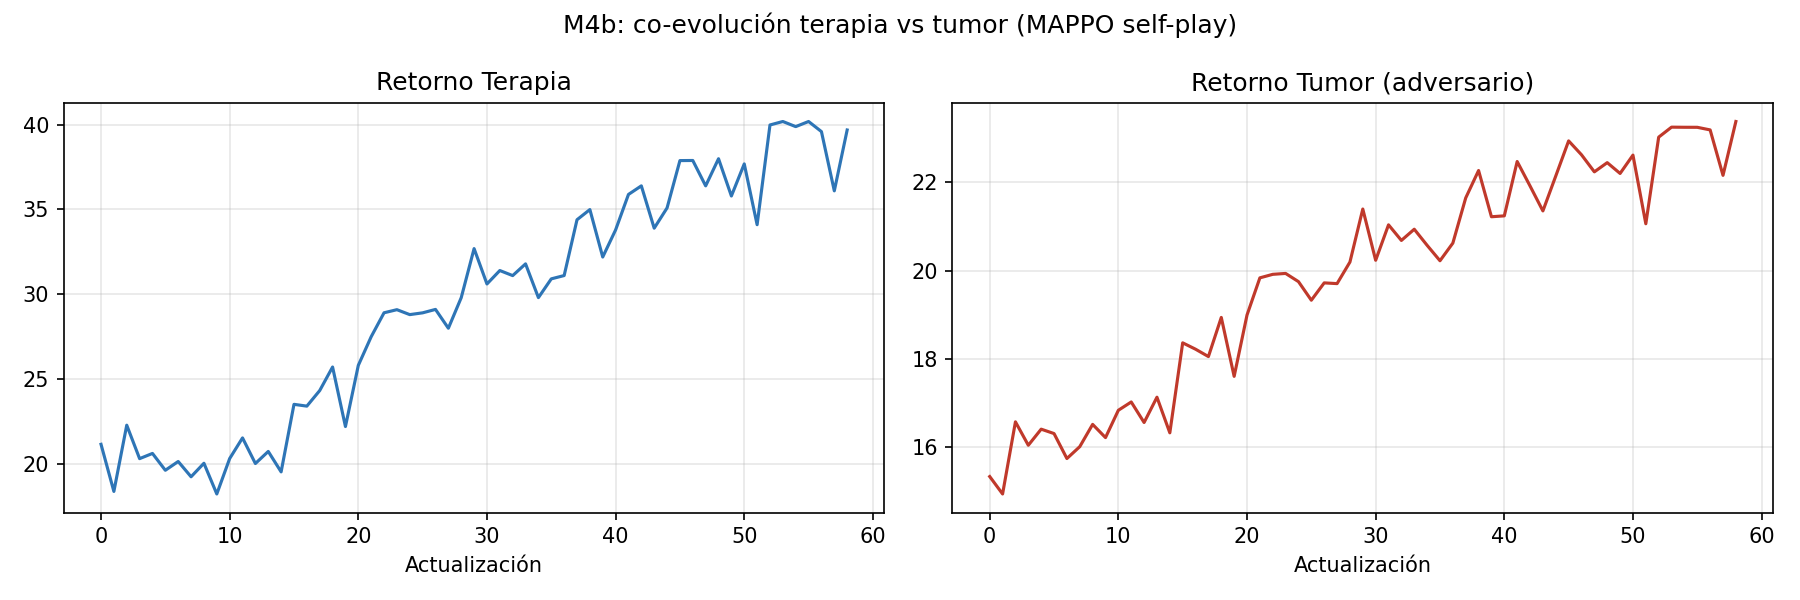
\includegraphics[width=0.95\textwidth]{images/mappo_learning_curves.png}
\caption{Curvas de aprendizaje del entrenamiento adversarial MAPPO por self-play: retorno del agente de terapia (izquierda) y del agente tumoral (derecha) a lo largo de las actualizaciones.}
\label{fig:learning}
\end{figure}

\section{Comparación frente a las líneas base}
\label{sec:res-comparacion}

La política aprendida se comparó contra tres referencias deterministas bajo la métrica de tiempo a falla combinado (TTP-combinado), reportando el modo de falla de cada estrategia. La Tabla~\ref{tab:res-baselines} resume los resultados de una evaluación representativa.

\begin{table}[H]
\centering
\caption{Comparación de estrategias bajo la métrica TTP-combinado, con el modo de falla. Métrica auditada mediante el procedimiento de diagnóstico.}
\label{tab:res-baselines}
\renewcommand{\arraystretch}{1.25}
\begin{tabular}{l|c|c|c|l}
\textbf{Estrategia} & \textbf{TTP (días)} & \textbf{Carga final} & \textbf{Frac.\ R final} & \textbf{Modo de falla} \\
\hline
Sin tratamiento     & 12  & 0.80 & 0.12 & carga progresó \\
MTD (dosis máx.)    & 13  & 0.09 & 0.52 & resistencia mayoría \\
Gatenby (adaptativa)& 27  & 0.38 & 0.53 & resistencia mayoría \\
MAPPO (aprendida)   & 41  & 0.79 & 0.51 & resistencia mayoría \\
\end{tabular}
\end{table}

Dos observaciones se desprenden de la Tabla~\ref{tab:res-baselines}. Primero, la métrica auditada revela que la ausencia de tratamiento falla por progresión de carga (día 12) mientras la fracción resistente permanece baja (0.12); todas las estrategias que tratan fallan, en cambio, por mayoría resistente. Segundo, la dosis máxima reduce la carga al mínimo (0.09) pero falla casi tan rápido como la ausencia de tratamiento (día 13), confirmando que la reducción agresiva del tumor precipita la resistencia. La política aprendida por MAPPO alcanza el mayor tiempo de manejo (41 días en esta corrida), superando a la heurística de Gatenby (27 días) y a la dosis máxima (13 días). La Figura~\ref{fig:ttp} muestra las trayectorias de carga tumoral y de fracción resistente para las cuatro estrategias.

\begin{figure}[H]
\centering
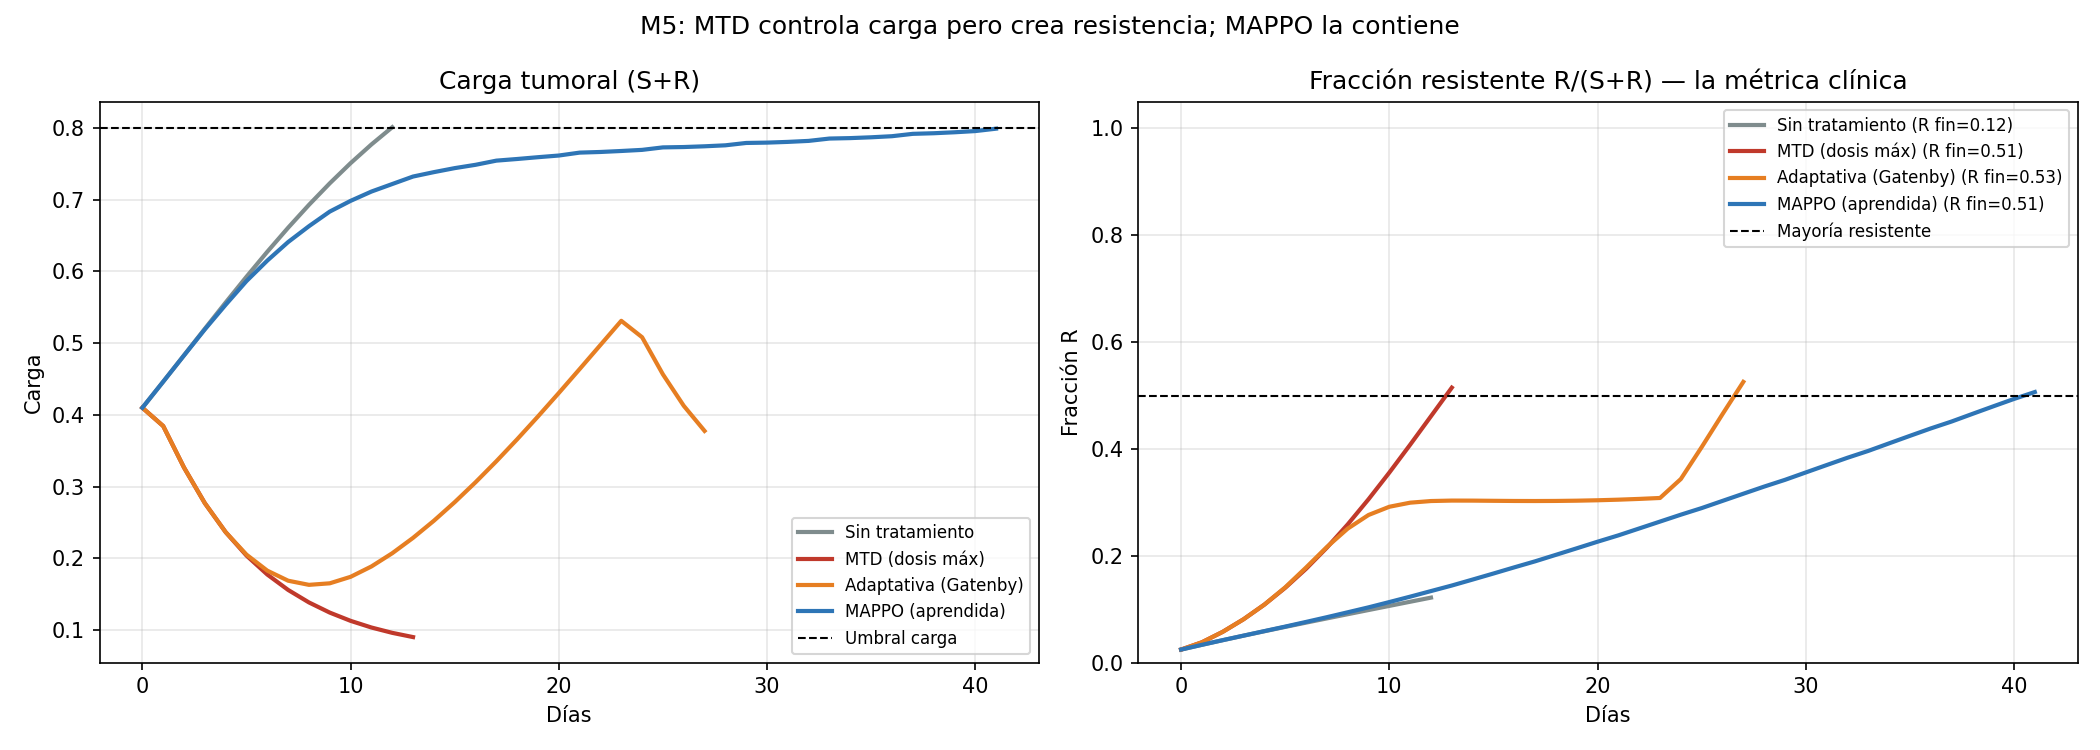
\includegraphics[width=0.95\textwidth]{images/evaluation_ttp.png}
\caption{Trayectorias de carga tumoral (izquierda) y de fracción resistente (derecha) para las cuatro estrategias. La dosis máxima controla la carga pero lleva la resistencia a su totalidad; la política aprendida retrasa la dominancia resistente.}
\label{fig:ttp}
\end{figure}

\subsection{Validación multi-semilla y bimodalidad}

Dado que el entrenamiento adversarial por \emph{self-play} es estocástico, el resultado se validó sobre 15 semillas independientes. La distribución de los tiempos de manejo es \textbf{bimodal}: una fracción de las corridas converge a una cuenca con tiempos en el rango de 25 a 33 días, mientras que otra fracción alcanza una cuenca superior, en torno a los 41 días. Reportamos por tanto ambos valores con igual peso: la \textbf{mejor corrida alcanza 41 días}, y la \textbf{media sobre las 15 semillas es de $33{,}5 \pm 5{,}8$ días} (mediana 32). La bimodalidad refleja que la co-evolución se asienta en distintos equilibrios según la inicialización, un fenómeno conocido del aprendizaje multiagente por self-play.

En ambas lecturas, la política aprendida supera a las dos líneas base de forma estadísticamente significativa (Tabla~\ref{tab:res-multisemilla}): frente a Gatenby ($p < 0{,}001$) y frente a la dosis máxima ($p < 0{,}001$). La Figura~\ref{fig:validation} muestra la comparación con barras de error.

\begin{table}[H]
\centering
\caption{Validación multi-semilla ($n=15$) del TTP-combinado. Las líneas base son deterministas. Significancia de la política aprendida frente a cada línea base.}
\label{tab:res-multisemilla}
\renewcommand{\arraystretch}{1.25}
\begin{tabular}{l|c|c}
\textbf{Estrategia} & \textbf{TTP (días)} & \textbf{Significancia} \\
\hline
MTD (dosis máx.)     & 13                       & --- \\
Gatenby (adaptativa) & 27                       & --- \\
MAPPO (mejor corrida)& 41                       & --- \\
MAPPO (media, $n=15$)& $33{,}5 \pm 5{,}8$ (mediana 32) & $p<0{,}001$ vs.\ MTD y Gatenby \\
\end{tabular}
\end{table}

\begin{figure}[H]
\centering
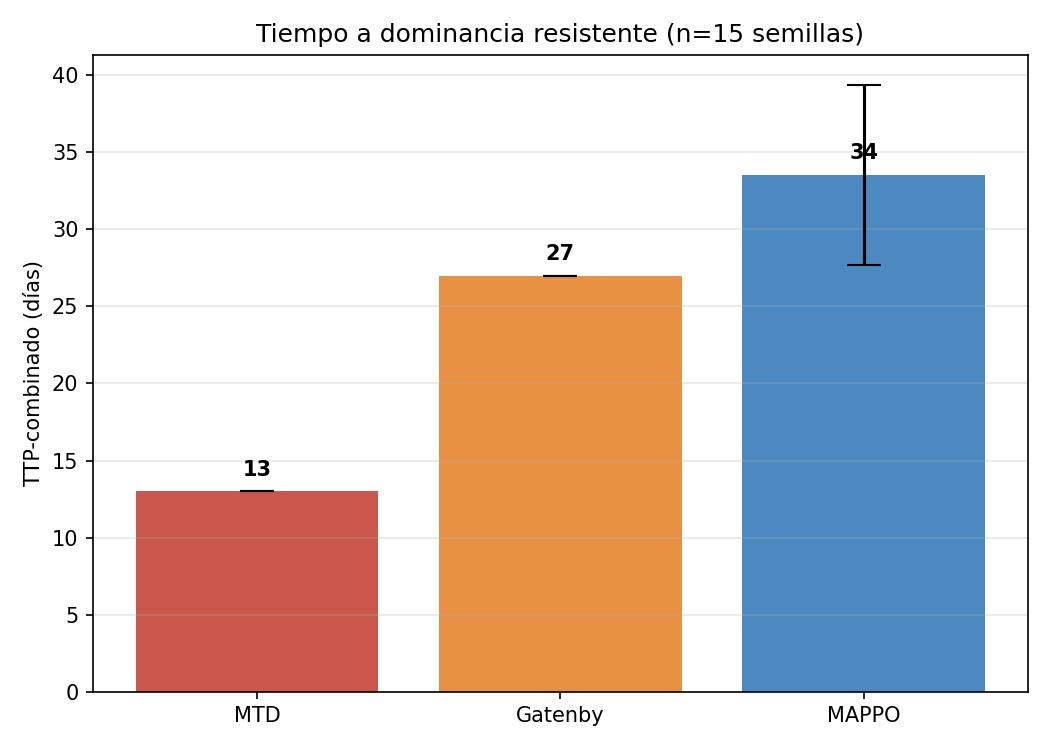
\includegraphics[width=0.6\textwidth]{images/validation_seeds.png}
\caption{Validación multi-semilla del TTP-combinado ($n=15$). La política aprendida supera a ambas líneas base deterministas; la barra de error refleja la dispersión bimodal del self-play.}
\label{fig:validation}
\end{figure}

\section{Mecanismo de la política aprendida}
\label{sec:res-mecanismo}

La inspección de las políticas de la cuenca superior revela el mecanismo descubierto por el agente. La Figura~\ref{fig:mecanismo} muestra que la política aplica una \textbf{dosificación pulsada e intermitente}: tras un periodo inicial, la dosis oscila entre valores bajos y nulos en lugar de mantenerse al máximo. Como consecuencia, la población sensible se mantiene en una densidad elevada que compite con la resistente y frena su expansión, mientras la fracción resistente crece lentamente hasta cruzar el umbral de mayoría. Este patrón corresponde al principio de la terapia adaptativa ---preservar una población sensible competidora--- redescubierto de forma autónoma por el agente, sin haber sido programado explícitamente.

\begin{figure}[H]
\centering
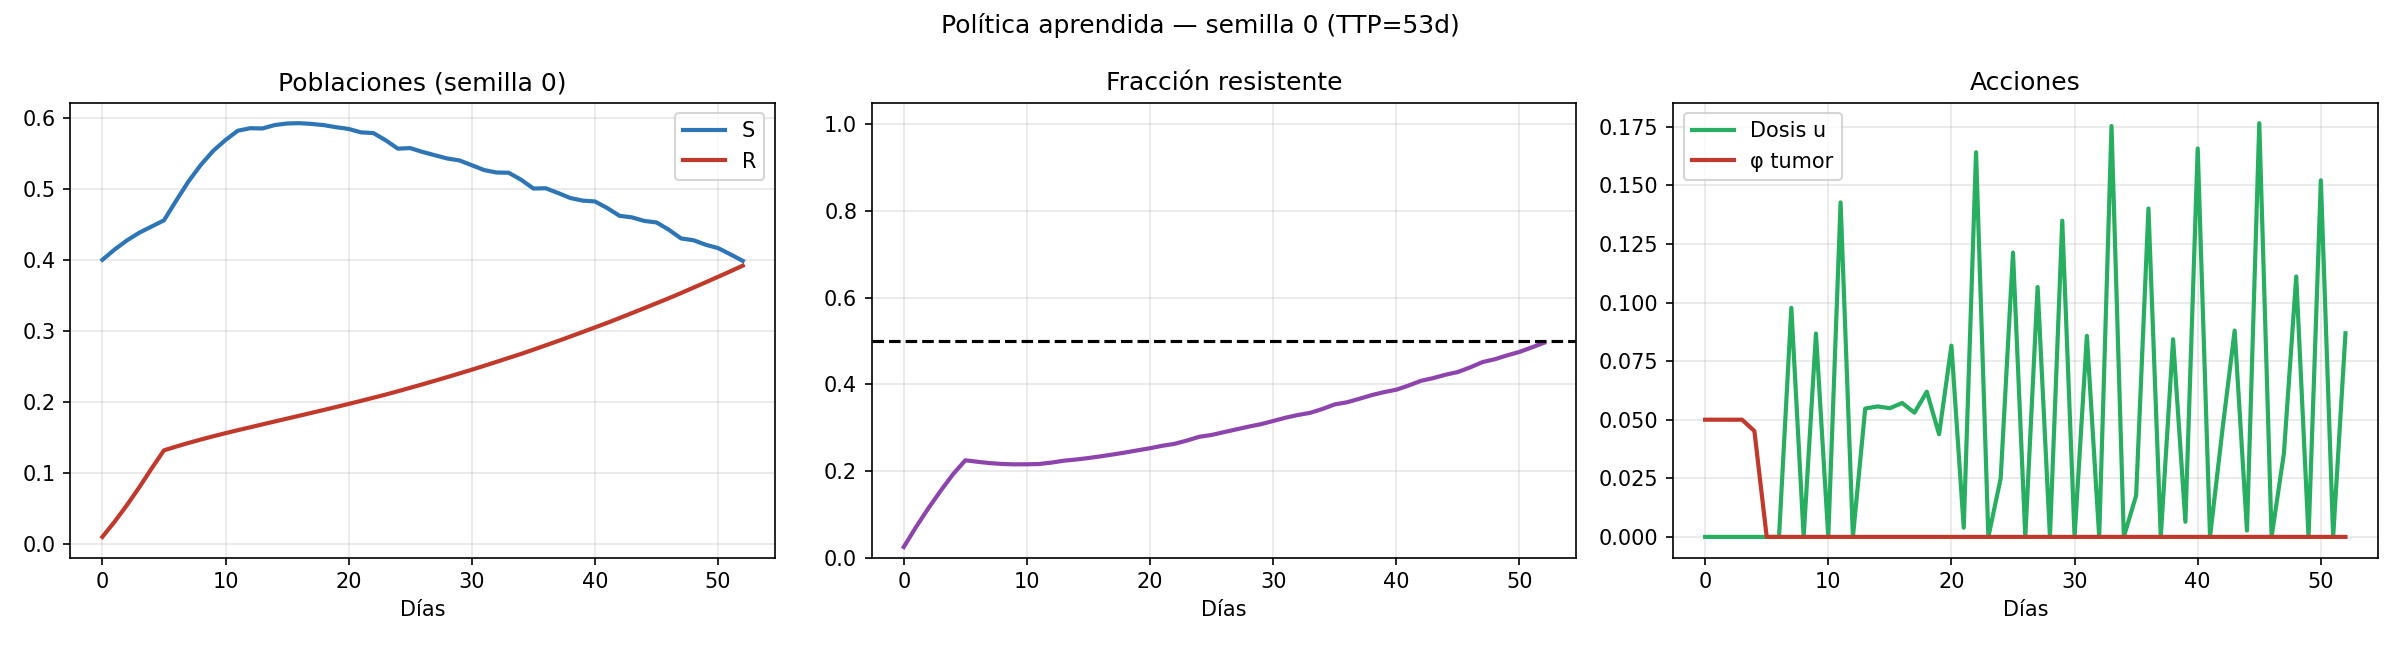
\includegraphics[width=0.95\textwidth]{images/policy_seed0.png}
\caption{Política aprendida de la cuenca superior: poblaciones (izquierda), fracción resistente (centro) y acciones de dosis y transición (derecha). La dosificación pulsada preserva la población sensible competidora.}
\label{fig:mecanismo}
\end{figure}

\section{Ablación del crítico centralizado (CTDE vs.\ IPPO)}
\label{sec:res-ablacion}

Para aislar la contribución del crítico centralizado, se comparó MAPPO (crítico condicionado al estado conjunto) con IPPO (crítico con observación local), manteniendo idénticos el actor, la observación de ejecución y todos los hiperparámetros. La verificación de la arquitectura confirmó que el cambio de variante modifica efectivamente la dimensión de entrada del crítico (3 para MAPPO, 2 para IPPO).

Bajo la métrica auditada, MAPPO alcanza un tiempo de manejo medio de $34{,}8 \pm 5{,}7$ días frente a $30{,}2 \pm 2{,}9$ días de IPPO (Tabla~\ref{tab:res-ablacion}). La diferencia favorece al crítico centralizado, aunque su margen es estrecho. Un contraste cualitativo es informativo: las corridas de IPPO tienden a fallar por progresión de carga, mientras que las mejores corridas de MAPPO fallan por mayoría resistente, lo que indica que MAPPO sostiene el control de la carga durante más tiempo antes de ceder a la resistencia.

\begin{table}[H]
\centering
\caption{Ablación del crítico centralizado. Ambas variantes comparten actor, observación de ejecución e hiperparámetros; solo difiere la entrada del crítico.}
\label{tab:res-ablacion}
\renewcommand{\arraystretch}{1.25}
\begin{tabular}{l|c|l}
\textbf{Variante} & \textbf{TTP (días)} & \textbf{Modo de falla predominante} \\
\hline
MAPPO (crítico centralizado, CTDE) & $34{,}8 \pm 5{,}7$ & resistencia mayoría \\
IPPO (crítico local)               & $30{,}2 \pm 2{,}9$ & carga progresó \\
\end{tabular}
\end{table}

\begin{figure}[H]
\centering
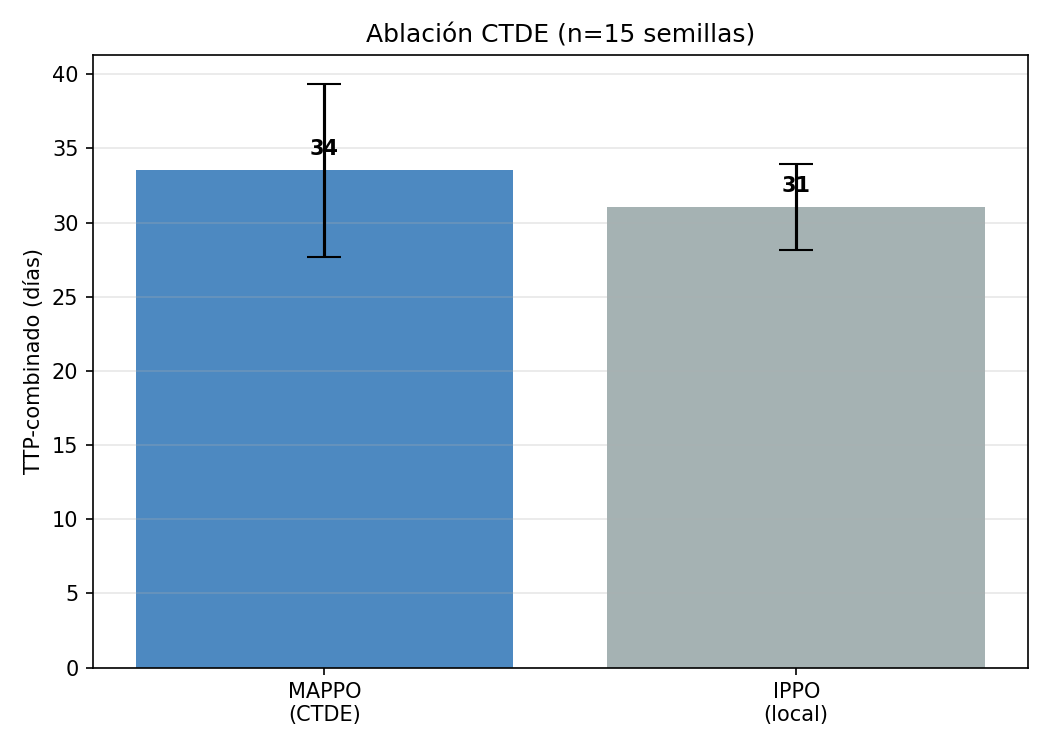
\includegraphics[width=0.6\textwidth]{images/ablation_ctde.png}
\caption{Ablación CTDE: MAPPO (crítico centralizado) frente a IPPO (crítico local) bajo el TTP-combinado.}
\label{fig:ablacion}
\end{figure}

\section{Análisis de sensibilidad}
\label{sec:res-sensibilidad}

Se varió, una a la vez, cada una de las seis constantes elegidas a mano alrededor de su valor por defecto, recalculando el TTP-combinado de las tres estrategias en cada punto. La Tabla~\ref{tab:res-sensibilidad} resume el rango de la política aprendida frente a las líneas base. En las seis constantes y en todo el rango evaluado, la política aprendida se mantiene por encima de la heurística de Gatenby y de la dosis máxima; el ordenamiento $\text{MAPPO} > \text{Gatenby} > \text{MTD}$ no se invierte en ningún punto.

\begin{table}[H]
\centering
\caption{Análisis de sensibilidad. Rango del TTP-combinado de MAPPO al variar cada constante $\pm 30\%$ (o entre valores razonables), frente al rango de las líneas base.}
\label{tab:res-sensibilidad}
\renewcommand{\arraystretch}{1.25}
\begin{tabular}{l|c|c|c}
\textbf{Constante variada} & \textbf{MAPPO (rango)} & \textbf{Gatenby} & \textbf{MTD} \\
\hline
$\phi_{\max}$ (fuerza adversario)    & 30.0--39.3 & 27        & 13 \\
$\theta_{\text{prog}}$ (umbral carga)& 32.3--44.0 & 27        & 13 \\
$\rho_{\text{may}}$ (umbral mayoría) & 28.3--40.3 & 25--29    & 11--15 \\
$w_{\text{tox}}$ (toxicidad)         & 37.7       & 27        & 13 \\
$\delta_S^{\max}$ (potencia fármaco) & 33.7--38.3 & 27--29    & 10--19 \\
$\mathrm{IC50}_R$ (brecha resistencia)& 36.0--39.7 & 27--28   & 13--15 \\
\end{tabular}
\end{table}

El parámetro más sensible es la potencia del fármaco $\delta_S^{\max}$: al aumentarla, la dosis máxima falla más rápido (de 19 a 10 días) por selección acelerada de resistencia, mientras que la política aprendida y la heurística de Gatenby se mantienen estables. La Figura~\ref{fig:sensibilidad} presenta los seis barridos.

\begin{figure}[H]
\centering
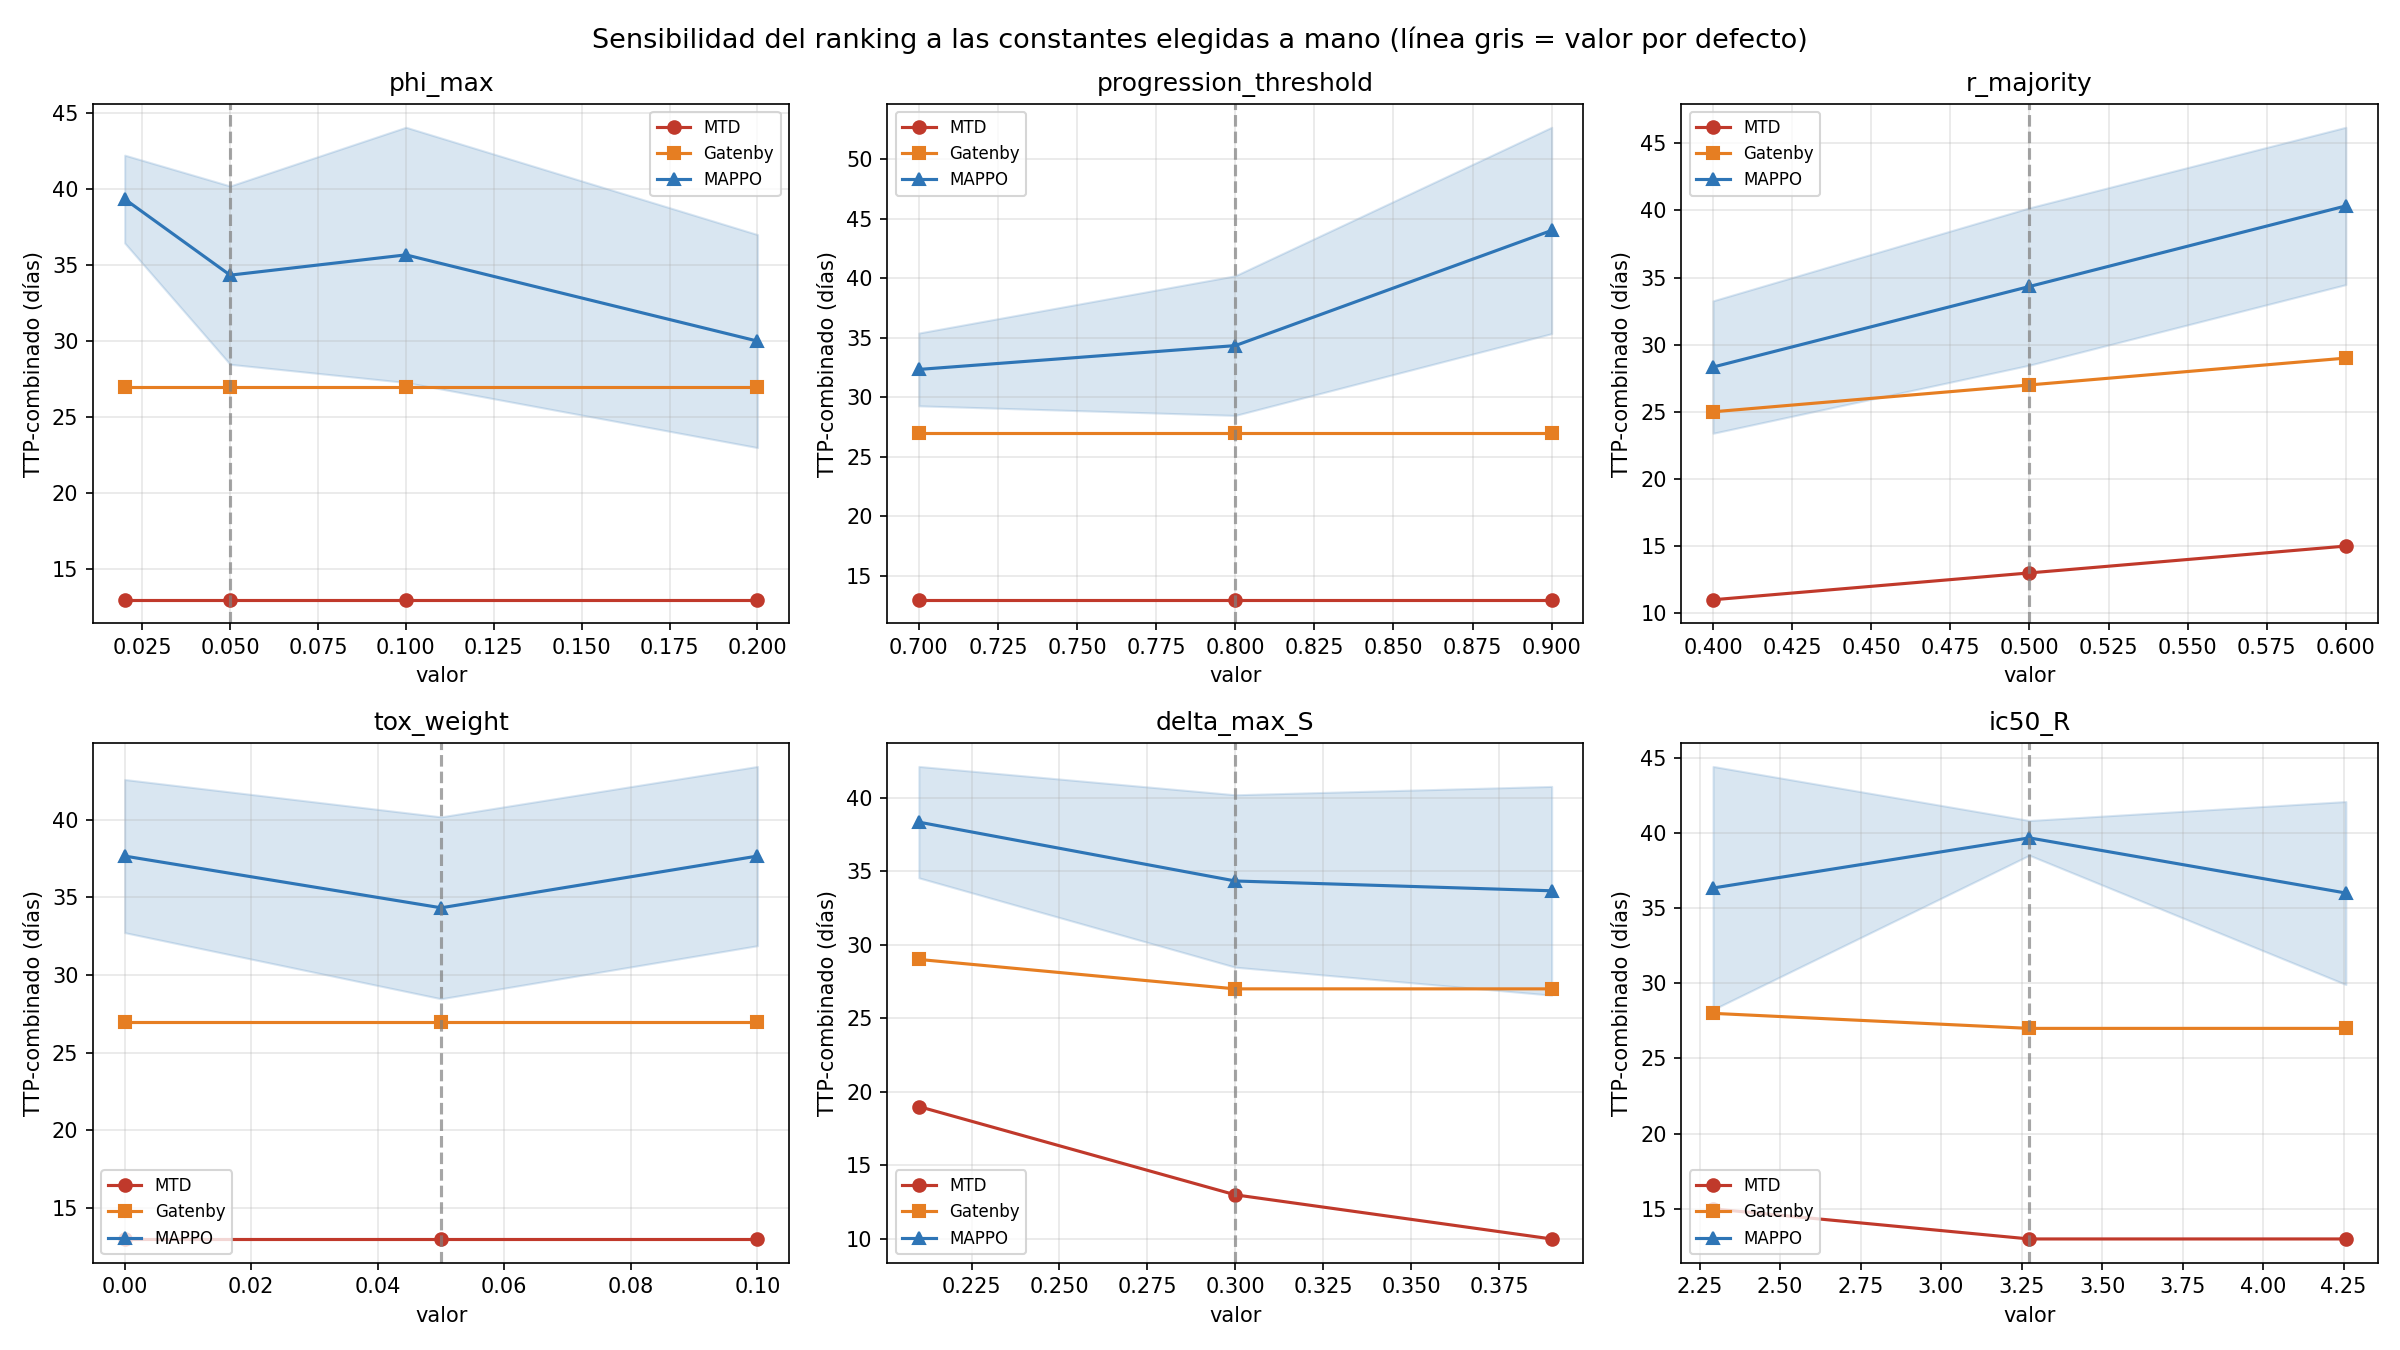
\includegraphics[width=0.95\textwidth]{images/sensitivity.png}
\caption{Análisis de sensibilidad sobre las seis constantes elegidas a mano. La curva de la política aprendida (azul) se mantiene por encima de Gatenby y de la dosis máxima en todo el rango; la línea vertical gris marca el valor por defecto.}
\label{fig:sensibilidad}
\end{figure}

\section{Confirmación con la corrida completa reproducible}
\label{sec:res-confirmacion}

Para verificar que los hallazgos no dependen de la maquinaria de cómputo, se reejecutó el pipeline completo de extremo a extremo bajo el arnés reanudable con checkpointing intra-corrida descrito en la Sección~\ref{sec:checkpointing}: el modelo titular y las dos ramas de la ablación se entrenaron a la escala plena de \textbf{120\,000 pasos}, con \textbf{cinco semillas independientes} por variante, y se evaluaron con la métrica TTP-combinado auditada. Las líneas base, al ser deterministas, reprodujeron sus valores de forma exacta (Sin tratamiento 12 días, MTD 13 días, Gatenby 27 días), lo que confirma la integridad de la reejecución.

La Tabla~\ref{tab:res-confirmacion} reporta el tiempo de manejo por semilla. La lectura honesta para una distribución bimodal es la \textbf{tasa de éxito} y la \textbf{mediana}, no el promedio. MAPPO-CTDE supera a la heurística de Gatenby en las \textbf{cinco de cinco} semillas (mediana 33 días, mejor corrida 41), mientras que IPPO lo hace en \textbf{cuatro de cinco} (mediana 30 días). El ordenamiento $\text{MAPPO} > \text{IPPO} > \text{Gatenby} > \text{MTD} > \text{Sin tratar}$ se mantiene, reproduciendo el hallazgo central de la validación multi-semilla ($n=15$) con una corrida totalmente reproducible.

\begin{table}[H]
\centering
\caption{Corrida completa reproducible (120\,000 pasos, $n=5$ semillas por variante). TTP-combinado por semilla y tasa de éxito frente a Gatenby (27 días). Para la distribución bimodal se reporta mediana y tasa de éxito, no media$\pm$desv.}
\label{tab:res-confirmacion}
\renewcommand{\arraystretch}{1.25}
\begin{tabular}{l|c|c|c|c|c|c|c}
\textbf{Variante} & \textbf{s0} & \textbf{s1} & \textbf{s2} & \textbf{s3} & \textbf{s4} & \textbf{Mediana} & \textbf{Éxito $>$Gatenby} \\
\hline
MAPPO (CTDE) & 41 & 32 & 31 & 33 & 41 & \textbf{33} & \textbf{5/5} \\
IPPO (local) & 31 & 29 & 25 & 30 & 40 & 30 & 4/5 \\
\end{tabular}
\end{table}

La Figura~\ref{fig:confirmacion} contrasta las medianas de ambas variantes de RL frente a las tres líneas base (panel a) y muestra la dispersión por semilla que evidencia la bimodalidad (panel b): ambas variantes presentan una mayoría de corridas agrupadas en torno a los 30--33 días y semillas aisladas que alcanzan la cuenca superior de 40--41 días, justificando el reporte por tasa de éxito en lugar de promedios. Coherente con el mecanismo descrito en la Sección~\ref{sec:res-mecanismo}, la dosis media aprendida en todas las semillas exitosas es baja (en torno a 0.05--0.06), confirmando la dosificación pulsada como patrón estable del aprendizaje.

\begin{figure}[H]
\centering
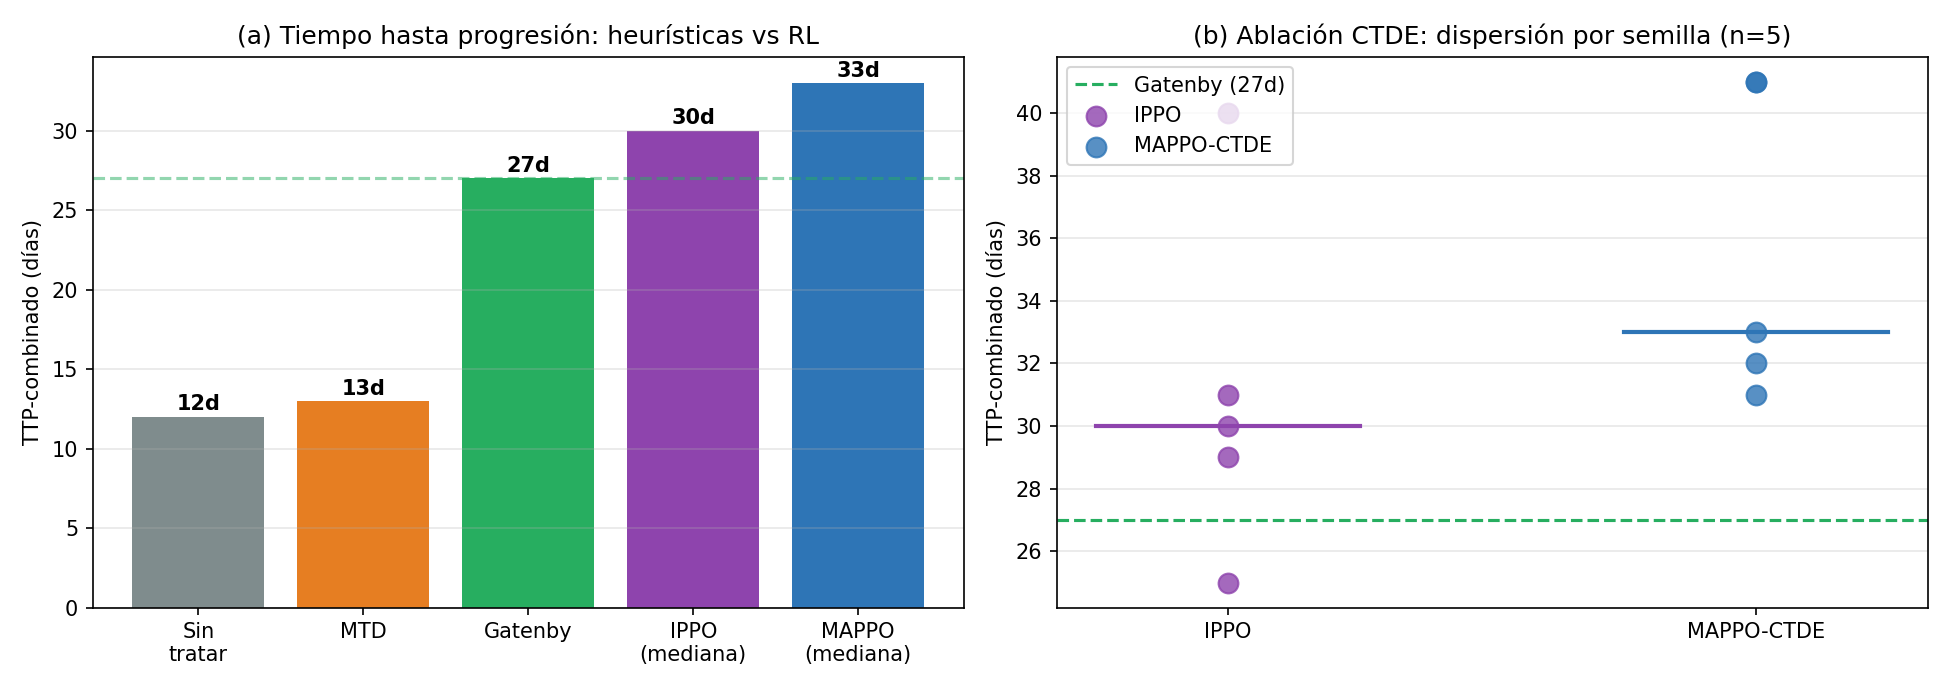
\includegraphics[width=\textwidth]{images/resultados_full_120k.png}
\caption{Corrida completa reproducible (120\,000 pasos). (a) Mediana del TTP-combinado de las variantes de RL frente a las líneas base; la línea discontinua marca a Gatenby. (b) Dispersión por semilla ($n=5$): la mayoría de corridas se agrupa cerca de la mediana y semillas aisladas alcanzan la cuenca superior (bimodalidad), por lo que el resultado se reporta como tasa de éxito.}
\label{fig:confirmacion}
\end{figure}

En conjunto, los resultados muestran que la política aprendida por GBMARL extiende el tiempo de manejo clínico de forma significativa frente a las dos líneas base, mediante un mecanismo de dosificación pulsada interpretable, con una ventaja modesta del crítico centralizado y un ordenamiento robusto frente a la variación de los hiperparámetros, y ese ordenamiento se reproduce en una corrida completa de extremo a extremo bajo control de reproducibilidad.